\videotitle{NASLib: A Modular and Extensible NAS Library}

%----------------------------------------------------------------------
\myframe{Motivation for NASLib \litw{Zela et al., 2020}}{

	\alert{NASLib} is a \alert{framework} for easily implementing different NAS methods, aiming to:
\medskip		
	\myit{
		\item Allow \alert{fair comparisons without confounding factors}, which could be due to 
		\myit{
			\item[-] Different codebases
			\item[-] Different search and evaluation pipelines
			\item[-] Different hyperparameter settings
			\item[-] Other confounding factors, e.g., library versions, GPU types, etc.
		}
\pause
\medskip
		\item \alert{Modularize} different components of NAS optimizers to allow combining them
			%, e.g. one can go from DARTS to GDAS by just a method call
\pause
\medskip
		\item Offer \alert{researchers} a convenient way of prototyping new NAS methods
\pause
\medskip
		\item Offer \alert{users} reliable implementations of NAS methods
		\myit{
			\item Facilitate the use of NAS for new search spaces
			\item Develop a robust true AutoML framework
		}
	}

}
%----------------------------------------------------------------------

%----------------------------------------------------------------------
\myframe{NASLib building blocks: Search Spaces, Optimizers, Evaluators}{
	\centering

	\myit{
		\item NASLib implements a broad range of NAS \alert{optimizers}
		\myit{
			\item \alert{Blackbox NAS methods}, e.g., Regularized Evolution
			\item \alert{One-shot NAS methods}, e.g., DARTS
		}
	}
	
\medskip
\pause	
	\myit{
		\item The \alert{optimizers are modularized}
		\myit{
			\item This allows to switch from, e.g., DARTS to GDAS or PC-DARTS by just one method call
		}

\medskip
\pause
		\item The \alert{evaluators are agnostic to the origin of an architecture}
		\myit{
			\item The final architecture is run using exactly the same object to evaluate on the test set
		}
	}
\medskip
\pause
	\myit{
		\item NASLib's main building block is the graph object represented as a \alert{NetworkX}~\only<4->{\footnote{https://networkx.github.io/}} graph
		\myit{
			\item[-] \alert{Easily manipulate the graph} by adding/removing nodes/edges 
			\item[-] \alert{Hide complexity} of dealing with the PyTorch computational graph
			\item[-] \alert{Easy high-level way of creating complex structures}, e.g., hierarchical search spaces
		}
	}
}
%----------------------------------------------------------------------

%----------------------------------------------------------------------
\myframe{NASLib building blocks: Search Spaces, Optimizers, Evaluators}{
	\myit{
		\item The \alert{optimizers are agnostic to the search space} they are running on 
		\myit{
			\item This facilitates their use for new types of search spaces
		}
\pause
\bigskip
		\item \alert{An optimizer takes the search space as a NetworkX object and builds the PyTorch computational graph}
	}
	\vspace*{-0.3cm}
	\begin{columns}
		\column{0.18\textwidth}
		\column{0.3\textwidth}
		\begin{center}
		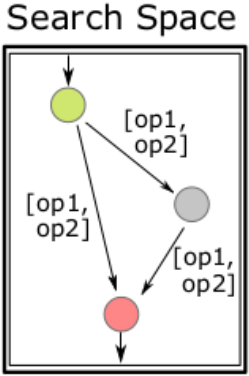
\includegraphics[width=0.35\textwidth]{images/naslib_space.png}	
		\end{center}
		
		\column{0.04\textwidth}
		~\\[23pt]\Huge{$\Rightarrow$}
	
		\column{0.3\textwidth}
		\begin{center}
		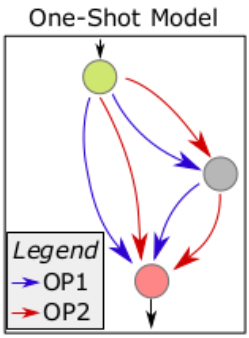
\includegraphics[width=0.4\textwidth]{images/naslib_oneshot_model.png}	
		\end{center}
	\column{0.18\textwidth}
	\end{columns}

\pause
\smallskip
	\myit{
		\item Depending on the optimizer, each operation choice in the NetworkX object becomes:
		\myit{
			\item[-] a $\texttt{MixedOp}$ -- for one-shot NAS optimizers, e.g. DARTS
			\item[-] a $\texttt{CategoricalOp}$ -- for black-box optimizers, e.g. Regularized Evolution
		}
	}
	
}
%----------------------------------------------------------------------

%----------------------------------------------------------------------
\myframe{NASLib: Overview}{
	\centering
	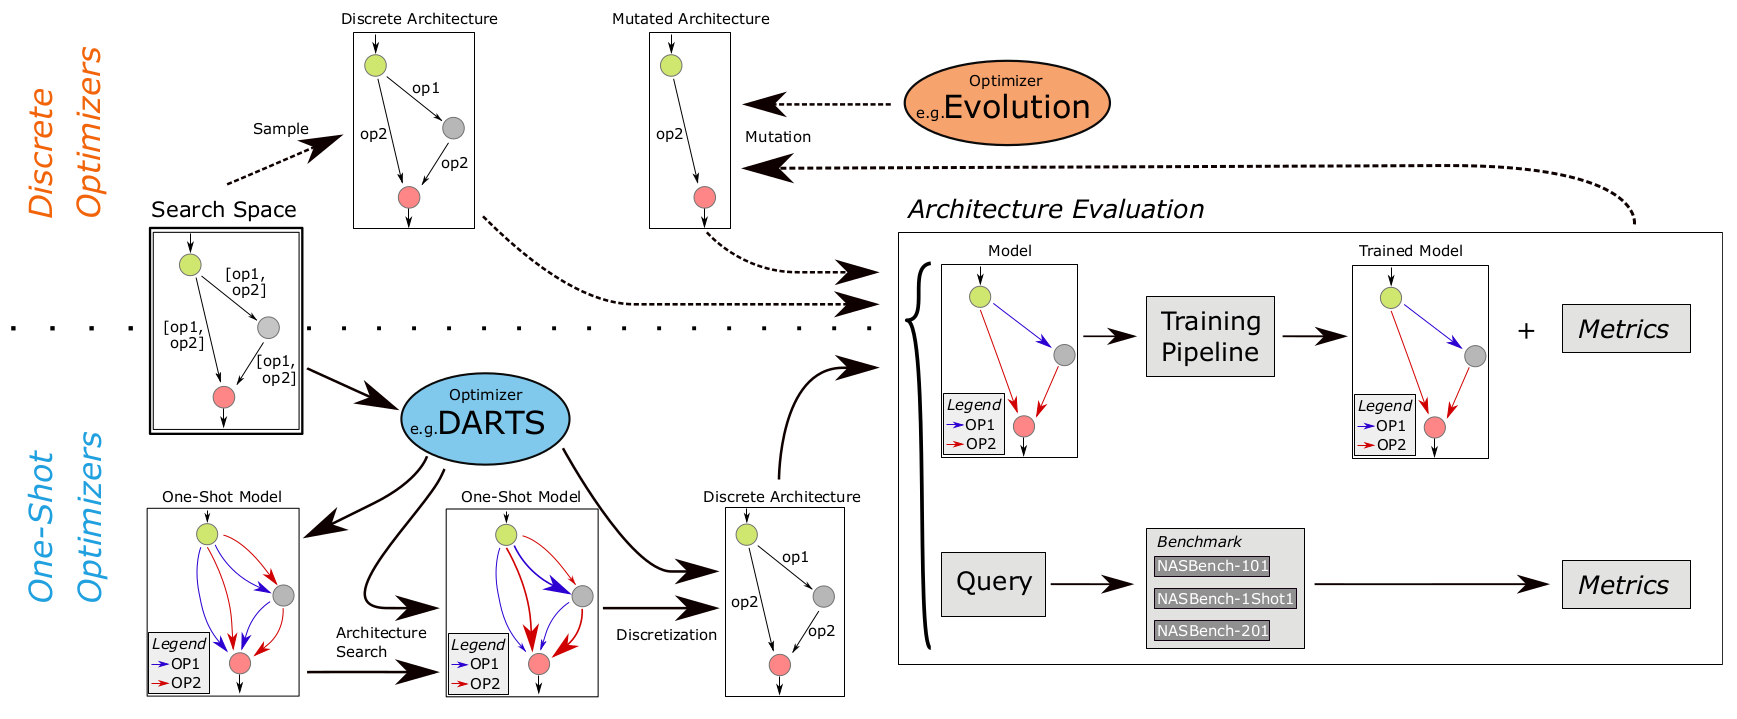
\includegraphics[width=0.85\textwidth]{images/naslib.png}\\	
}
%----------------------------------------------------------------------

\myframe{Tabular benchmarks for one-shot NAS}{
	\centering
	\myit{
		\item NAS-Bench-101 \lit{\href{https://arxiv.org/abs/1902.09635}{Ying et al. 2019}} is not directly compatible with one-shot NAS methods 
		\myit{
			\item Mainly due to the constraint of at most 9 edges in the cell
		}
		\bigskip
		\pause
		\item \alert{NAS-Bench-1Shot1} \lit{\href{https://openreview.net/forum?id=SJx9ngStPH}{Zela et al. 2020}}
		\myit{
				\item[-] \alert{3 sub-spaces of NAS-Bench-101} that are compatible with one-shot methods
				\myit{
					\item \alert{6\,240, 29\,160, and 363\,648 architectures}, respectively
				}
				\item[-] Currently the largest one-shot NAS tabular benchmark
			}
		\bigskip
		\pause
		\item \alert{NAS-Bench-201} \lit{\href{https://openreview.net/forum?id=HJxyZkBKDr}{Dong and Yang. 2020}}
		\myit{
%				\item[-] Same graph representation as in DARTS
				\item[-] Much smaller than NAS-Bench-101 and largest NAS-Bench-1Shot1 subspace
				\myit{
					\item \alert{15\,625 architectures}
				}
				\item[-] Every architecture in the search space evaluated on \alert{3 image classification datasets}
			}
		}
}
%----------------------------------------------------------------------
%----------------------------------------------------------------------
\myframe{NASLib case study: Results on NAS-Bench-201}{
	\centering
	\begin{minipage}{.4\textwidth}
		\myit{
			\item<1-> NAS-Bench-201 is already integrated in NASLib and we can run any one-shot optimizer on it
\medskip
			\item<2-> We can also combine random perturbations \lit{\href{https://arxiv.org/pdf/2002.05283.pdf}{Chen and Hsieh, 2020}} with any one-shot optimizer
\medskip
			\item<3-> We can also evaluate black-box optimizers cheaply with a tabular benchmark
		}	
	\end{minipage}
	\begin{minipage}{.58\textwidth}
		\centering
		\visible<1->{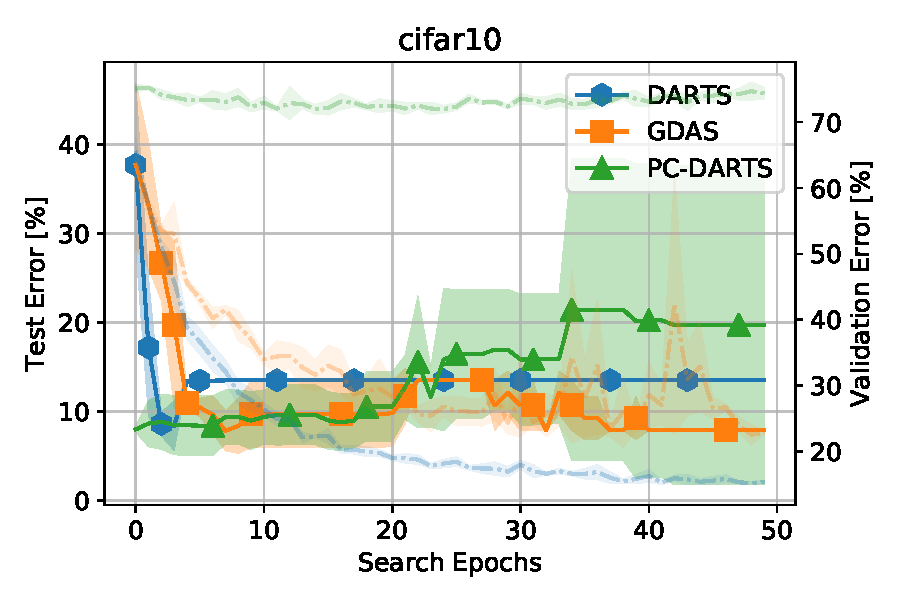
\includegraphics[width=0.45\textwidth]{images/nb201_1.pdf}}
		\visible<2->{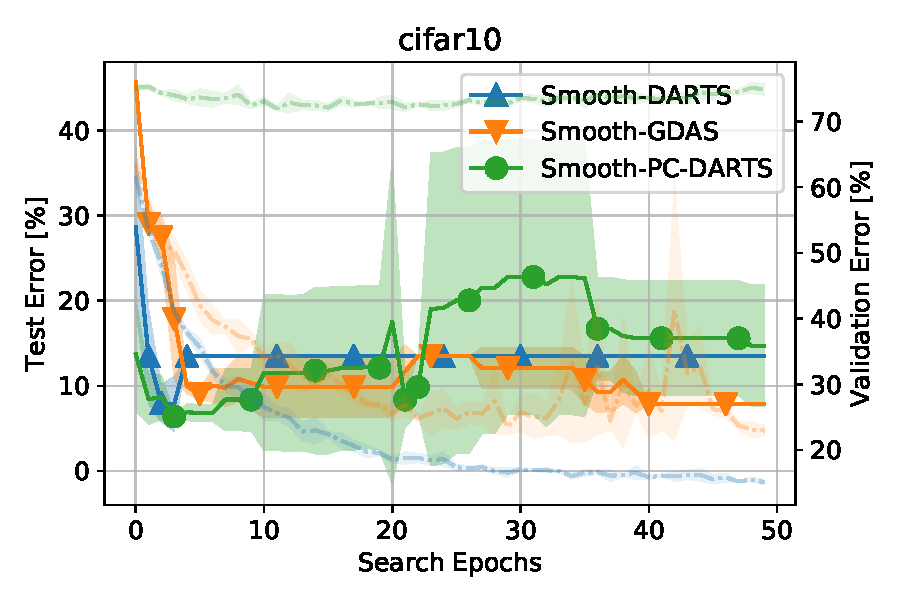
\includegraphics[width=0.45\textwidth]{images/nb201_2.pdf}}\\
		\visible<3->{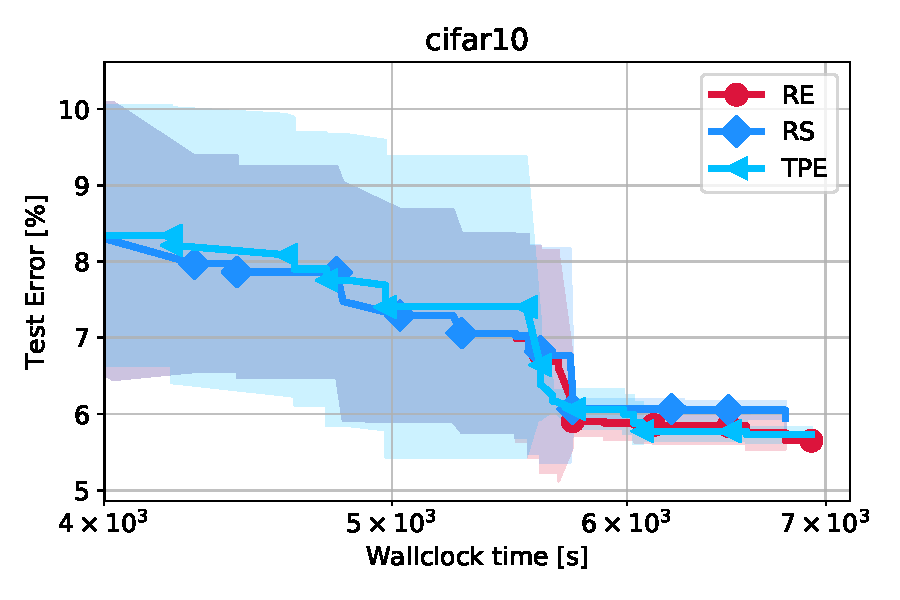
\includegraphics[width=0.55\textwidth]{images/nb201_3.pdf}}
	\end{minipage}	
}

%----------------------------------------------------------------------

%----------------------------------------------------------------------
\myframetop{Opportunities with NASLib}{
	\alert{Room for many interesting projects and theses}
	\myit{
		\item Applications of NAS to \alert{your problem of interest}, with interesting search spaces
		\myit{
			\item NASLib is the first library that separates the NAS method from the search spaces
			\myit{
				\item Therefore, \alert{no changes are required in the NAS methods}
				\item This should make new applications much easier
			}
		}
	
\pause
\medskip
		\item Studying \alert{hierarchical search spaces} in detail
\pause
\medskip
		\item \alert{Combining different components} of existing NAS methods
		\myit{
			\item So far, it has been very hard on a code level to mix and match components
			\item It ought to be possible to design the world's best NAS method by combining the right components
		}
\pause
\bigskip
	}
	\alert{Room for interesting Hiwi projects} 
	\myit{
		\item Not everything is perfect yet, we can use lots of support by great programmers
	}
}

%----------------------------------------------------------------------



%----------------------------------------------------------------------
\myframe{Questions to Answer for Yourself / Discuss with Friends}{

	\myit{
		\item Repetition:\\ \alert{What would one have to do in order to apply the methods in NASLib to a new search space?}
\bigskip
		\item Discussion:\\ \alert{Is there a problem of your interest that you would you like to apply the methods in NASLib to?}
\bigskip
		\item Discussion:\\ \alert{Given that NASLib's modular design allows mixing and matching components of one-shot NAS methods, which of the methods we discussed might make sense to combine?}
	}	 
}
%-----------------------------------------------------------------------



